% !TEX root = ../../thesis.tex
\tikz[remember picture,overlay] \node[inner sep=0pt] at (current page.center){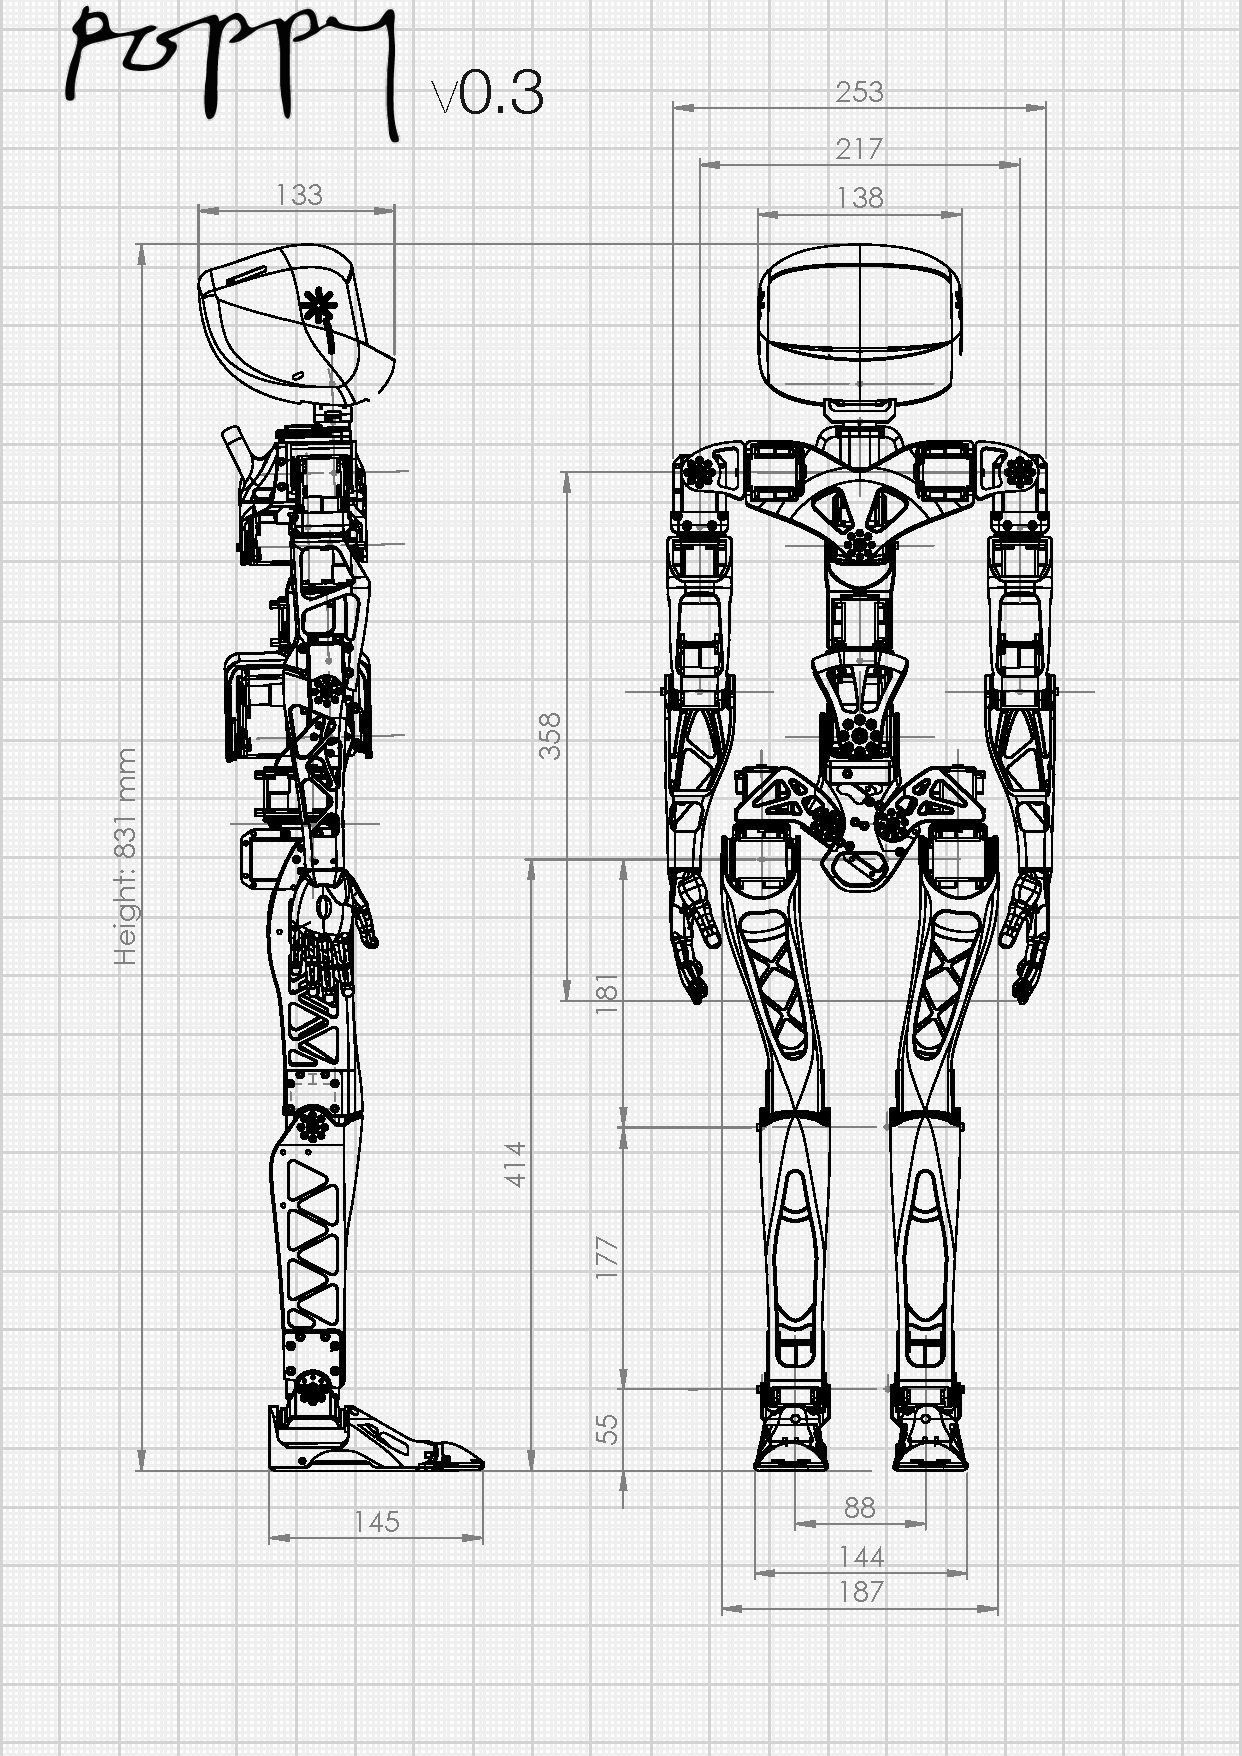
\includegraphics[width=\paperwidth,height=\paperheight]{Poppy_dimensions}};
\clearpage

\section{A little robot} % (fold)
\label{sec:poppy-little-robot}

To reach the goals presented in the introduction, the size of the robot is a really important aspect.

On one hand, small size makes the integration of complex, powerful and accurate mechatronics very difficult. Therefore, it reduces the scope of technology we could use for the robot. In particular, the integration of hydraulic and pneumatic actuators, as well as advanced mechanisms involving several moving parts is really challenging.

On the other hand, having a small robot is really convenient for exploring morphological properties in the real world.

Firstly, it changes significantly the experimental process: the ratio between weight, and thus energy and torques enforced by movements, and the mechanical robustness of the structure and of the actuators, is such that the robot can fall without breaking itself. Moreover, it is lightweight, which allows people to handle it directly without additional infrastructure and in a safe way. On the one hand, all of this speeds up the experimental process. On the other hand, it deeply changes the methodology of movement and motor skill design by allowing the creation of movements directly on the robot by real-world experiments without a simulation process. This includes for instance adjusting motor primitives in real time, even critical ones.

Secondly, this brings advantages regarding human interaction, which is an important focus in this work: on one hand, from the above reasons, this rules out the problem of physical security in Human/Robot interaction. On the other hand, the size of the robot plays an important role in the psychological representation that people have of it.

However exploring morphological properties requires having a robot that morphology has an actual impact on its dynamic. Being too small reduces this impact because it reduces the inertia and the role of intrinsic structural frequency.

Thus Poppy's size is a compromise to facilitate at the same time easy testing in the real world, the integration of a large number of degrees of freedom (25 DoFs) and a structure those dynamic properties cannot be neglected.

\subsection{Morphological proportions} % (fold)

From an anatomical point of view, Poppy reproduces the human proportions as described in the literature~\parencite{dufour2005biomecanique} (see \figurename~\ref{fig:poppy-human-proportion}) and the sensorimotor space organization: i.e. the main degrees of freedom (actuated and passive).

As the human grows from child to adult, his body proportions change~\parencite{bogin2010leg}. One hypothesis we made is that human proportions converge toward an optimal link ratio. Based on this hypothesis, we decided to respect the human body proportion of an adult, thus the size of the robot described previously (see section~\ref{sec:poppy-little-robot}) has defined all\footnote{An exception was made for the head, which is bigger to make it cuter and will be discussed in section~\ref{sec:head-design}.} dimensions  of Poppy's links with the proportions presented on \figurename~\ref{fig:poppy-human-proportion}.

\begin{figure}[tb]
    \centering
        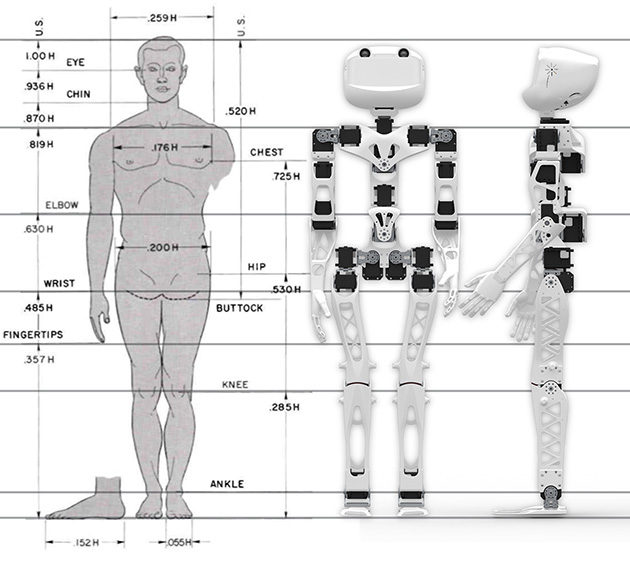
\includegraphics[width=0.8\linewidth]{proportion_poppy.jpg}
    \caption{Human proportion used for the design of Poppy~\parencite{dufour2005biomecanique}}
    \label{fig:poppy-human-proportion}
\end{figure}

Of course, this hypothesis is contestable, and, for example, mimicking the proportions of a child the same size as Poppy could be as relevant. Yet this choice has been taken as a starting point. Thanks to the design methodology we have and the open source diffusion, anyone can easily explore other choices and compare them.

\subsection{Small and lightweight feet} % (fold)

With the goal of achieving biped locomotion, most humanoid robots have big, flat and rectangular feet. This design is indeed really convenient to simplify balance problems while easily increasing the sustentation polygon, but this design choice carries some constraints:

Firstly, increasing the foot size increases the lever arm applied to the ankle. It can be useful as it extends the impact of the ankle control over the whole body. Yet given the potential high-torque applied to the ankle, achieving such control requires very powerful actuators.
Powerful actuators are heavier and, therefore, the whole actuation design of the robot needs to be powerful in order to be able to lift and move the feet.

Secondly, some interesting dynamic controllers for biped locomotion seem to require mass-less legs~\parencite{hyon2002development}. Indeed, in this case, there is no moment of inertia due to the motion of the legs, therefore controlling the whole body is simplified. While this case is a theoretical trick, it can still be transferred to the real world if there are a strong trunk/legs mass ratio. Therefore, either the overall mass of the robot should increase in order to make the mass of the legs negligible or we should design more lightweight legs.
Because they are the furthest element from the torso, the mass of the feet has a strong impact on the inertia of the legs.

Finally, while current state of the art robots show that it is still simpler to achieve biped locomotion with big and heavy feet, some projects show impressive results thanks to the use of small or flexible feet~\parencite{bruneau2001dynamic}. We can cite in particular Petman who demonstrates cutting-edge skills in biped locomotion over very complex terrain\footnote{Link youtube}.
Moreover, this aspect seems to be coherent with multi-legged animal species, indeed most animals have really thin legs and very small feet.

So even if common humanoid robots still use big and powerful feet, for the above-mentioned reasons, we decided to explore bio-inspired, small, and lightweight feet (see \figurename~\ref{fig:poppy-foot-v1-design}).



% \begin{figure}[p]
%     \centering
%         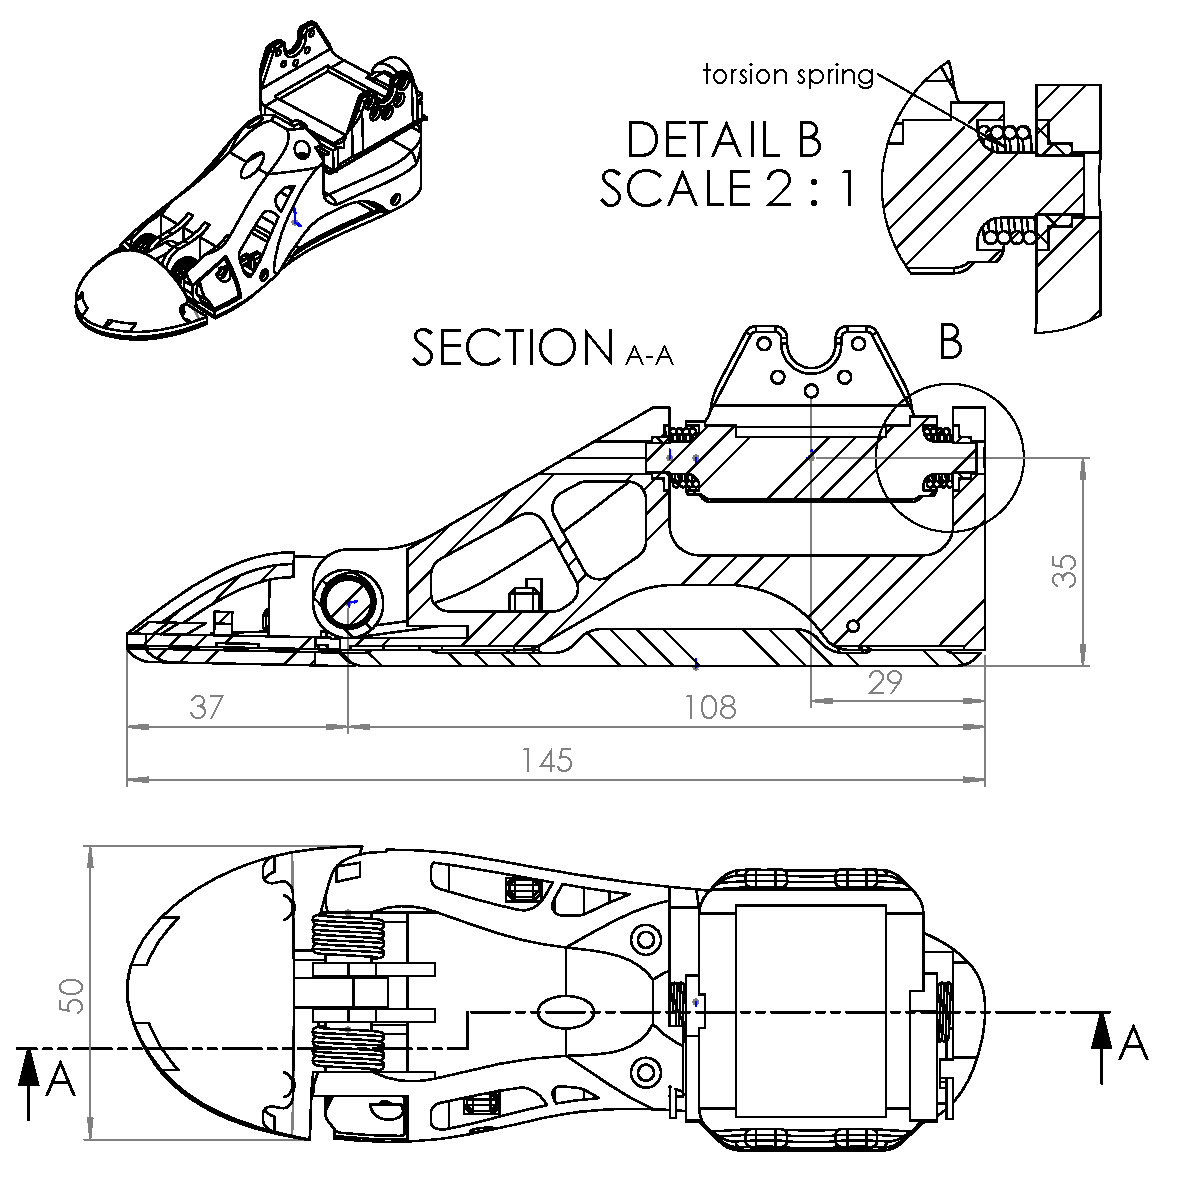
\includegraphics[width=\linewidth]{poppy_foot_v1.pdf}
%     \caption{Blueprint of Poppy's right leg. Parts have a truss structure to reduce the mass, and each leg has 6 DoF. Only the one on the hip use powerful motors (MX-64), others are powered by MX-28. This choice makes the robot could not support its weight if knees keep bended during walking. Therefore it constraints the research of more human-like gait with straight support leg.}
%     \label{fig:poppy_leg_design}
% \end{figure}

While the human foot is very complex system involving dozens of bones, muscles, and tendons, we simplified the design by extracting a few relevant functional human foot properties such as toes, which are key features concerning in both human walking~\cite{Hughes1990} and biped robots with a human-like gait~\cite{Sellaouti2006}. On Poppy's feet, to reduce the weight and complexity, we designed a passive articulation with torsion spring (see \figurename~\ref{fig:poppy-foot-v1-design}).
Also Poppy has very small feet compared to common humanoids, the ratio of height/length of feet is about 17\%,  close to the human one (see \figurename~\ref{fig:poppy-human-proportion}) while robots such as Nao have feet that represent 27\% of the height.

% (see table~\ref{tab:poppy_feet_compare}).

% \begin{table}[!ht]
% \centering
% \begin{tabular}{l| c c c c c}
%     & Human & Nao & Darwin Op & Nimbro-OP & Poppy \\
%     \hline
%     height (cm)     &   NA & 58 & 45 & 95 & 83\\
%     Foot length (cm) &  NA & 16 & 23 & 20 & 14.5\\
%     ratio (\%)      &   16 & 27 & 23 & 20 & 17\\
% \end{tabular}
% \caption{This table shows the classic height/foot size proportion used for the humanoid robotic platform. }
% \label{tab:poppy_feet_compare}
% \end{table}

Finally, unlike most humanoids, Poppy has only one active DoF. Indeed, while Poppy has small feet, it appears the actual moment it can transmit to the ground is really little for the lateral motion.


\begin{figure}[p]
    \centering
        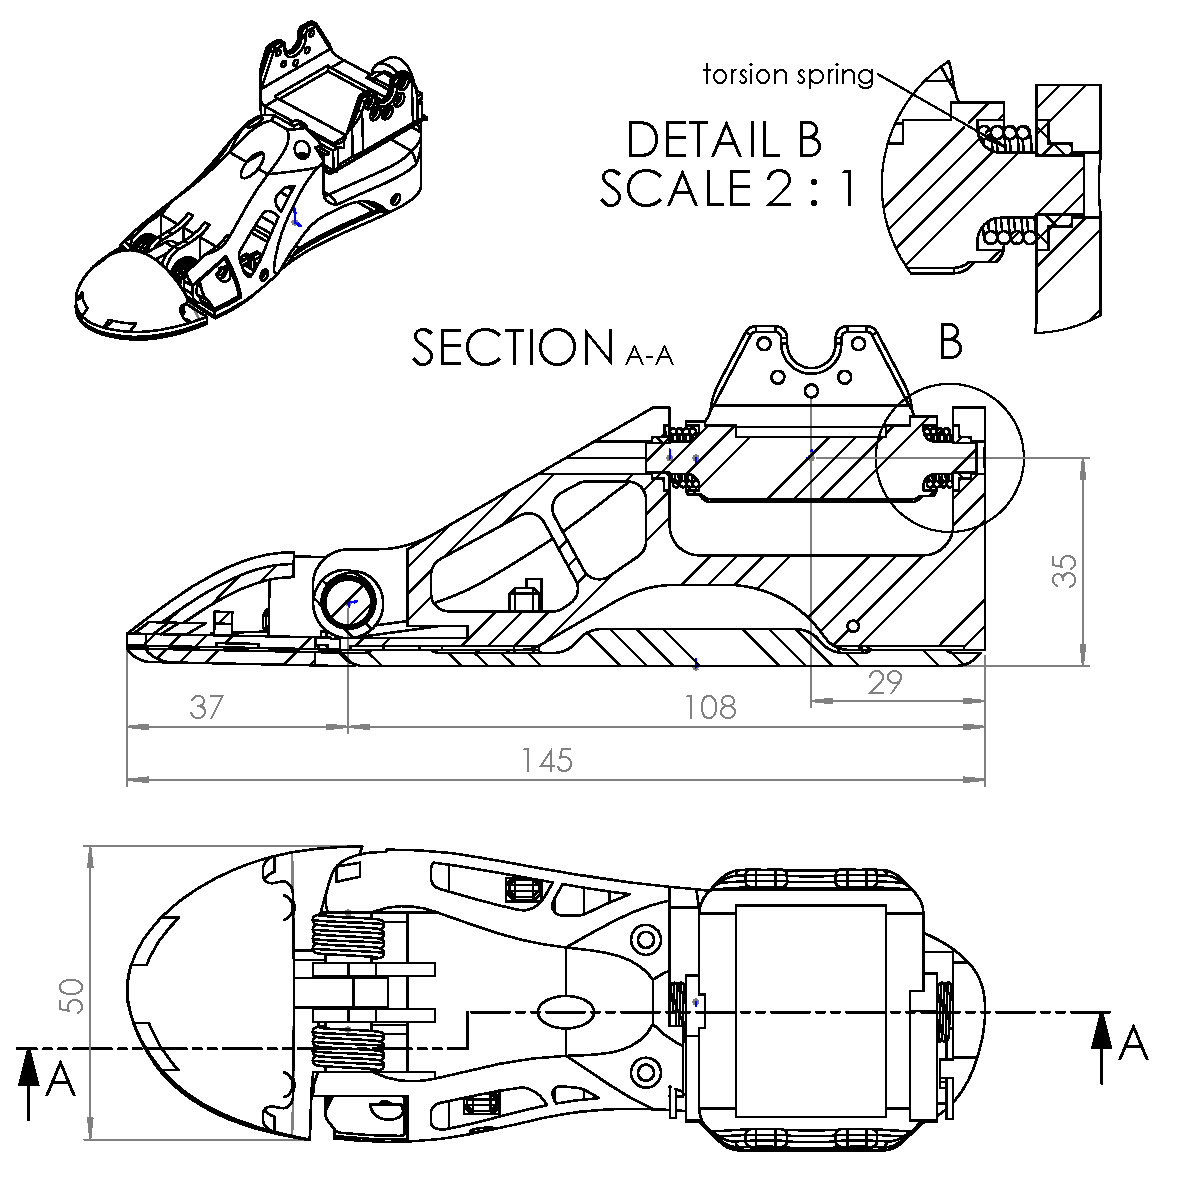
\includegraphics[width=\linewidth]{poppy_foot_v1.pdf}
    \caption{Blueprint of Poppy's foot. This foot has two passive joints, one for the toes, and one for the ankle roll. As we can see on the section A-A and detail B, both use torsion springs.}
    \label{fig:poppy-foot-v1-design}
\end{figure}

% \clearpage
Also creating an active articulation would add a lot of masses (72 gr) for little actual effect. Yet this DoF is still useful for ground adaptation.
We, therefore, preferred to design an articulation based on a passive joint with torsion springs (see \figurename~\ref{fig:poppy-foot-v1-design}).

This design choice has a strong impact on the overall design because we have lightweight feet, the power required to make the legs move is reduced, we can, therefore, use smaller motors which are also lighter.


% \begin{figure}[tb]
% \centering
%     \subfloat[][]{\label{fig:frontal_trunk}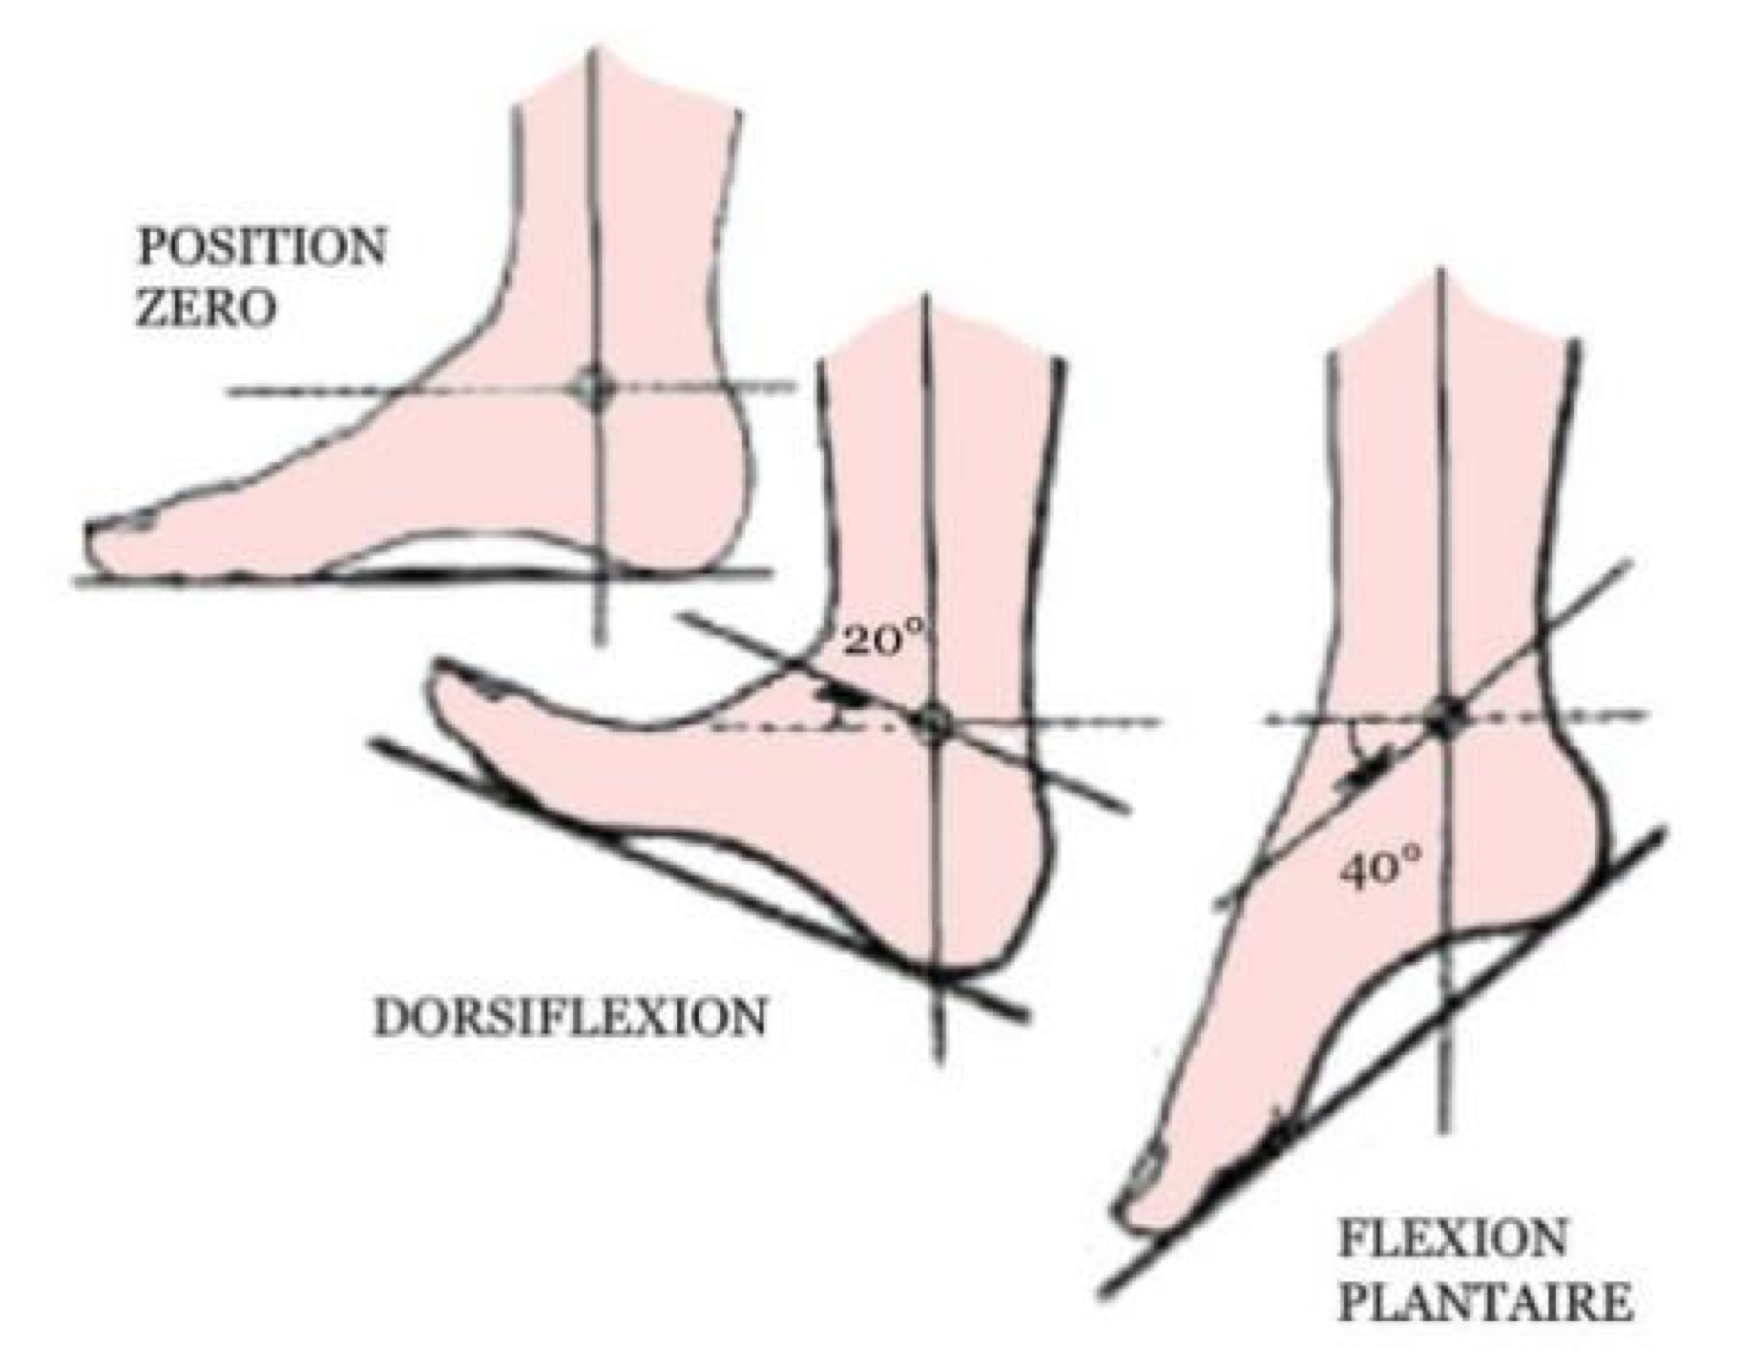
\includegraphics[height=4cm]{human_foot_sagittal.png}}
%     \hfil
%     \subfloat[][]{\label{fig:sagittal_trunk}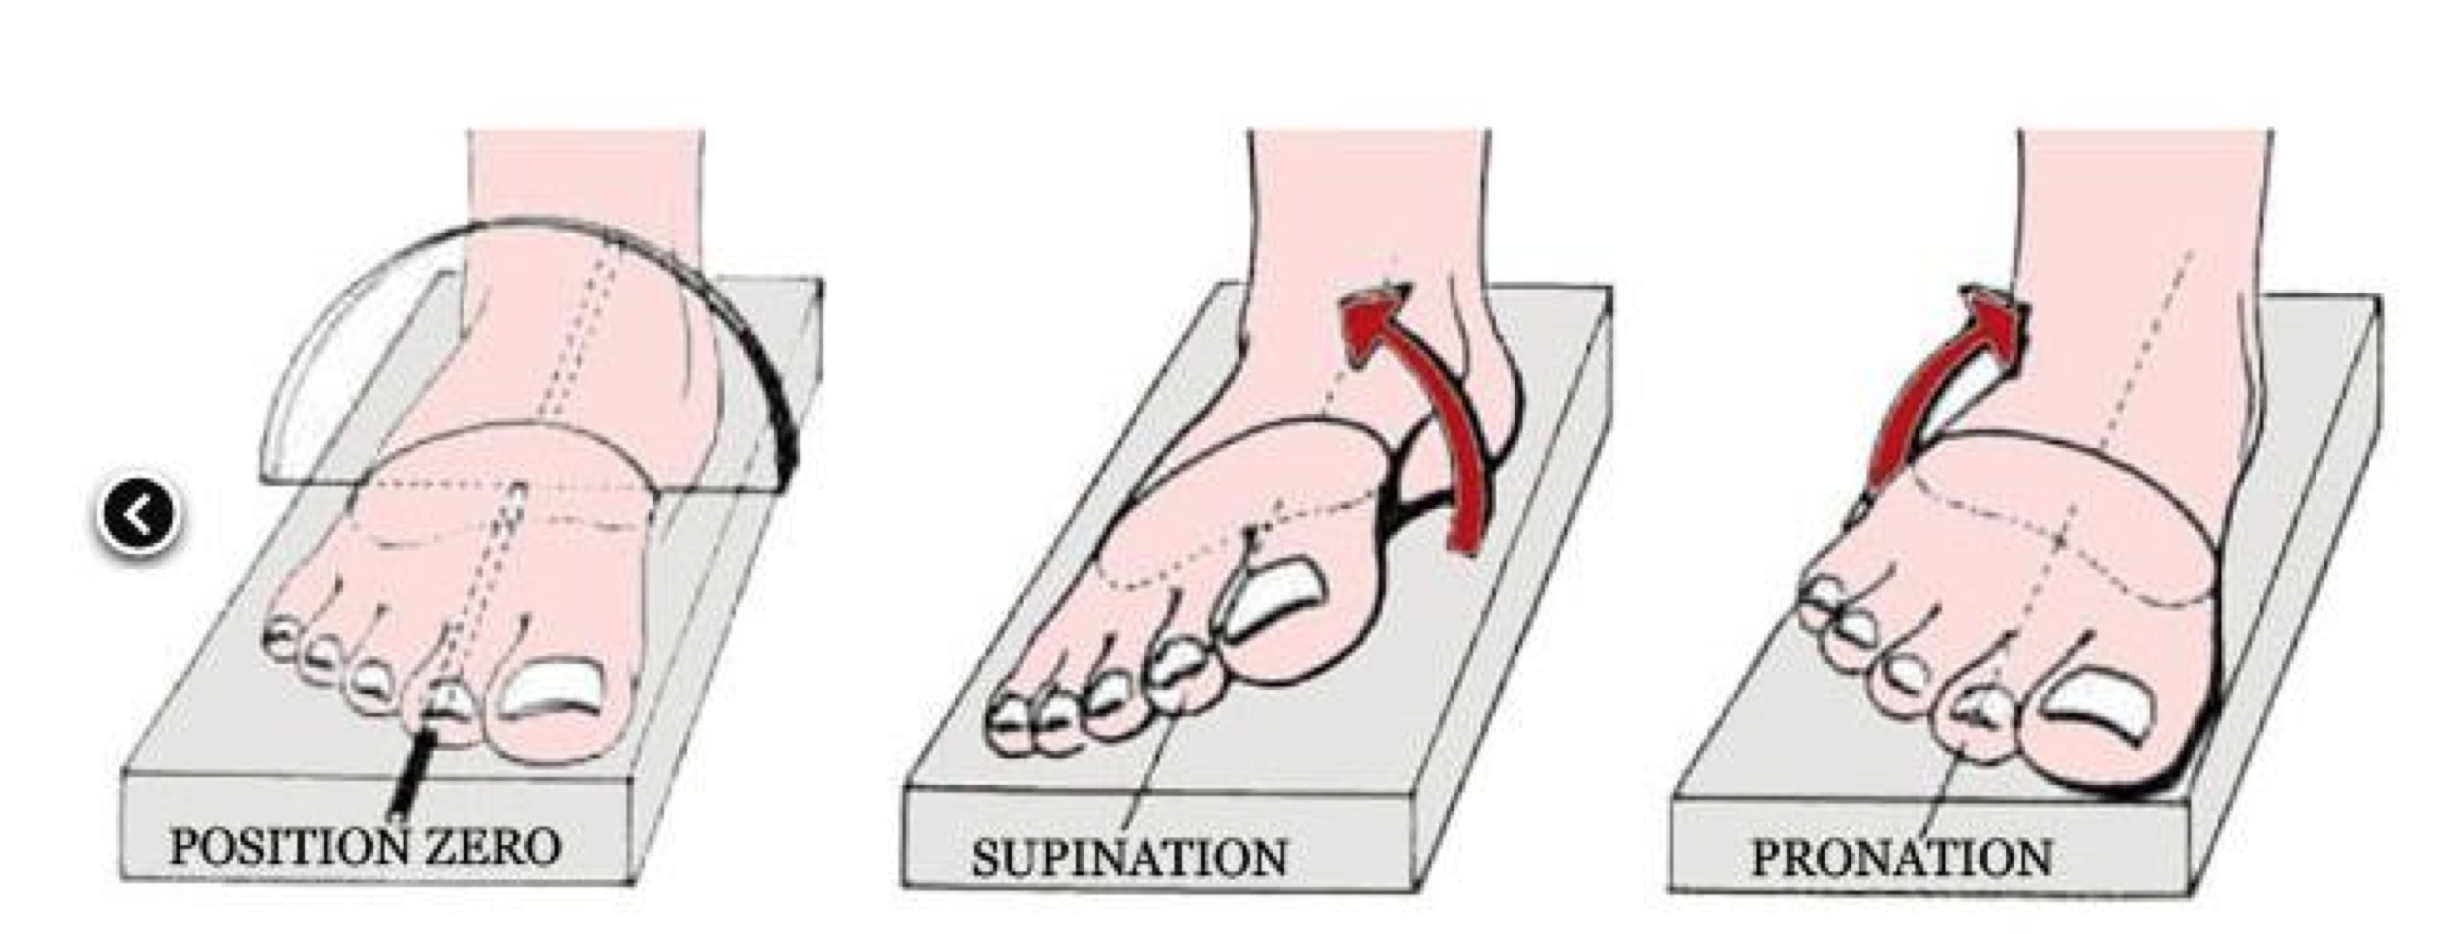
\includegraphics[height=3cm]{human_foot_lateral.png}}
%     \caption{}
%     \label{fig:poppy_torso}
% \end{figure}




\subsection{Legs} % (fold)
\label{sub:poppy-leg-design}

Poppy's legs have 6 DoF each, three on the sagittal plane (ankle, knee, hip), one on the horizontal plane (hip), and one on the frontal plane (hip). These joints allow reproduce the main DoF of the human legs. In addition, if we look closely at the morphology of the human femur, it appears that it is inclined by 6 degrees (see \figurename~\ref{fig:human_thigh_appendix}). This particularity is reproduced on Poppy's thigh (see \figurename~\ref{fig:poppy_leg_design}).

% \begin{figure}[tb]
% \centering
%     \subfloat[][]{\label{fig:human_thigh}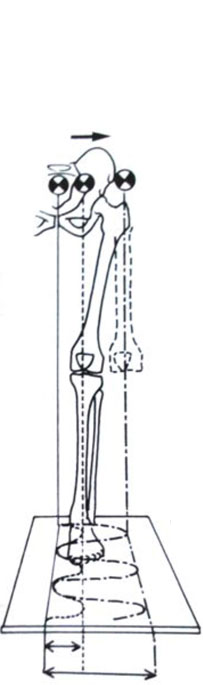
\includegraphics[height=6.5cm]{human_thigh.jpg}}
%     \hfil
%     \subfloat[][]{\label{fig:model_thigh}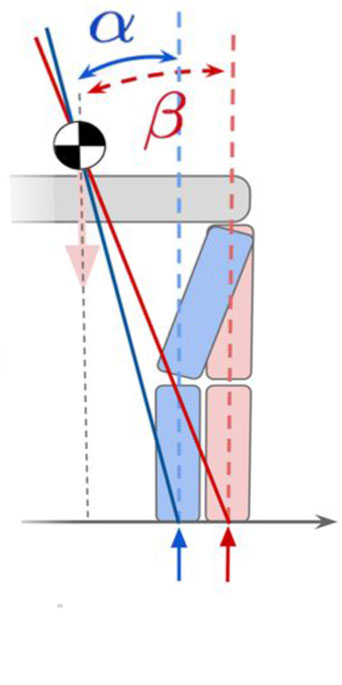
\includegraphics[height=6.5cm]{model_thigh.jpg}}
%     \caption{ On \ref{fig:human_thigh}, effect of the bended femur on human biped locomotion. \ref{fig:model_thigh} Model used for the morphological comparison of the two thighs.}
%     \label{fig:poppy_thigh}
% \end{figure}


This slight bending makes the feet closer to the projection of the center of gravity and, therefore, changes the dynamic behavior.
In this thesis we describe both a theoretical model (see appendix~\ref{appendix:thigh_model}) and real experiments (see section~\ref{sec:morphology-role}) showing that this bio-inspired thigh allows the reduction of falling speed by almost 60\% (during single support phase) and the decrease of the lateral motion needed for the mass transfer from one foot to the other by 30\% (double support phase).


\begin{figure}[p]
    \centering
        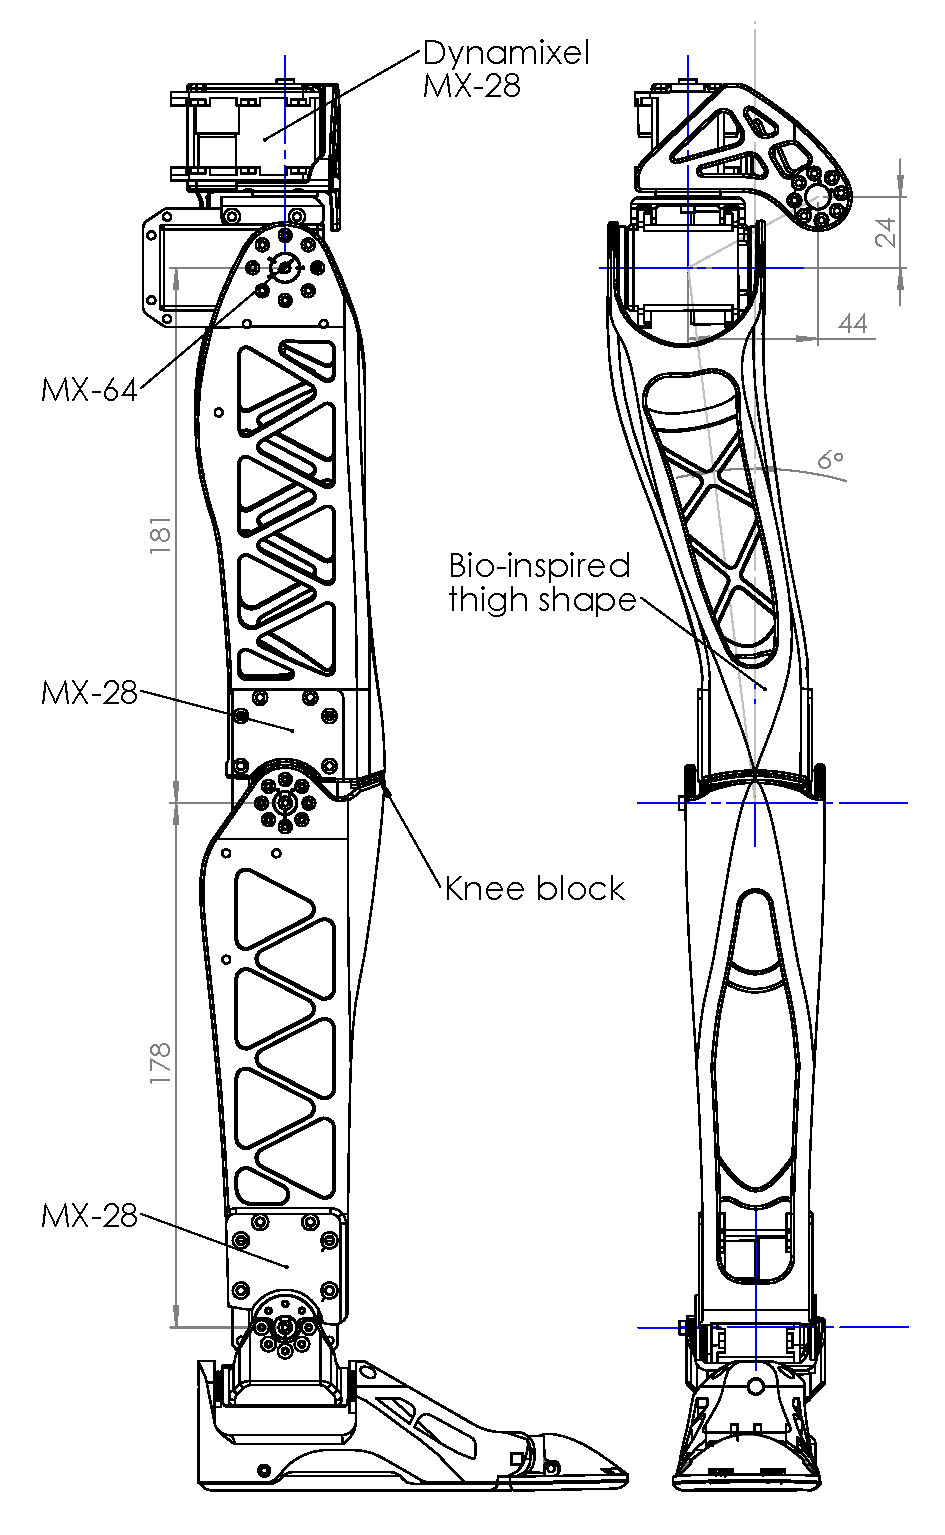
\includegraphics[width=0.97\linewidth]{poppy_leg_design.pdf}
    \caption{Blueprint of Poppy's right leg. Parts have a truss structure to reduce the mass, and each leg has 6 DoF. Only the one on the hip use powerful motors (MX-64), others are powered by MX-28. This choice makes the robot could not support its weight if knees keep bended during walking. Therefore it constraints the research of more human-like gait with straight support leg.}
    \label{fig:poppy_leg_design}
\end{figure}


Also, following the principles previously mentioned, the leg design is made to be as light as possible. This was achieved by using truss structure (see section~\ref{sec:lightweight-robot}) and the minimum required amount of power, involving two Dynamixel MX-28 for the ankle and knee joint, and a Dynamixel MX-64 for the hip joint (see \figurename~\ref{fig:poppy_leg_design}). Yet as explained in section REF, most of our parts have several configurations allowing the actuator to be changed. Thus, it is possible to easily replace the knee actuator by a Dynamixel MX-64 (see \figurename~\ref{sub:scalable-actuation}).


\section{Pelvis} % (fold)
\label{sec:hip}


Poppy's small feet increase the challenge of the balance of the robot. Also, to keep the projection of the center of gravity (CoG) inside the support polygon, defined by the feet geometry, it is necessary to control the weight distribution of the robotic structure. In particular, we wanted that in its initial upright posture, Poppy stays balanced without any control.

Robotis actuators are among the densest elements in the Poppy platform ($ 1700 kg.m^{3} $) and are the main source of weight ($1.8 kg$). Their spatial distribution represents, therefore, the major part of the distribution of mass in Poppy. In order to limit the displacement of the mass at the back of the robot, we decided to avoid a conventional ball joint assembly for the hip joint common on most robots based on Robotis motors such as DarwinOP or Acroban (i.e. distributed on a plane parallel to the sagittal plane). Instead, we placed them on the frontal plane as the left to right stability is greater than the rear to front stability. By doing so, the hip joint is not a real ball joint anymore. Yet to keep a wide range of motion, we used an original unsymmetrical motor configuration (see \figurename~\ref{fig:poppy_zoom_hip_blueprint}).

This configuration allows us:

\begin{itemize}
    \item to create a compact multi-articulated pelvis,
    \item have hip rotations (frontal plane) leading to slight vertical motions of the leg, which act as a damper during walking. This damping can be tuned by adjusting the stiffness of the actuator.
    \item to reduce the hip joint lever arm and thus reduce the torque required to maintain position in the single support phase,
    \item to reduce the distance between rotation axes to stay close to a ball joint,
    \item the resulting V shape frees up room to increase the range of motion of the legs on both the frontal and horizontal plane.
\end{itemize}

\begin{figure}[p]
    \begin{center}
        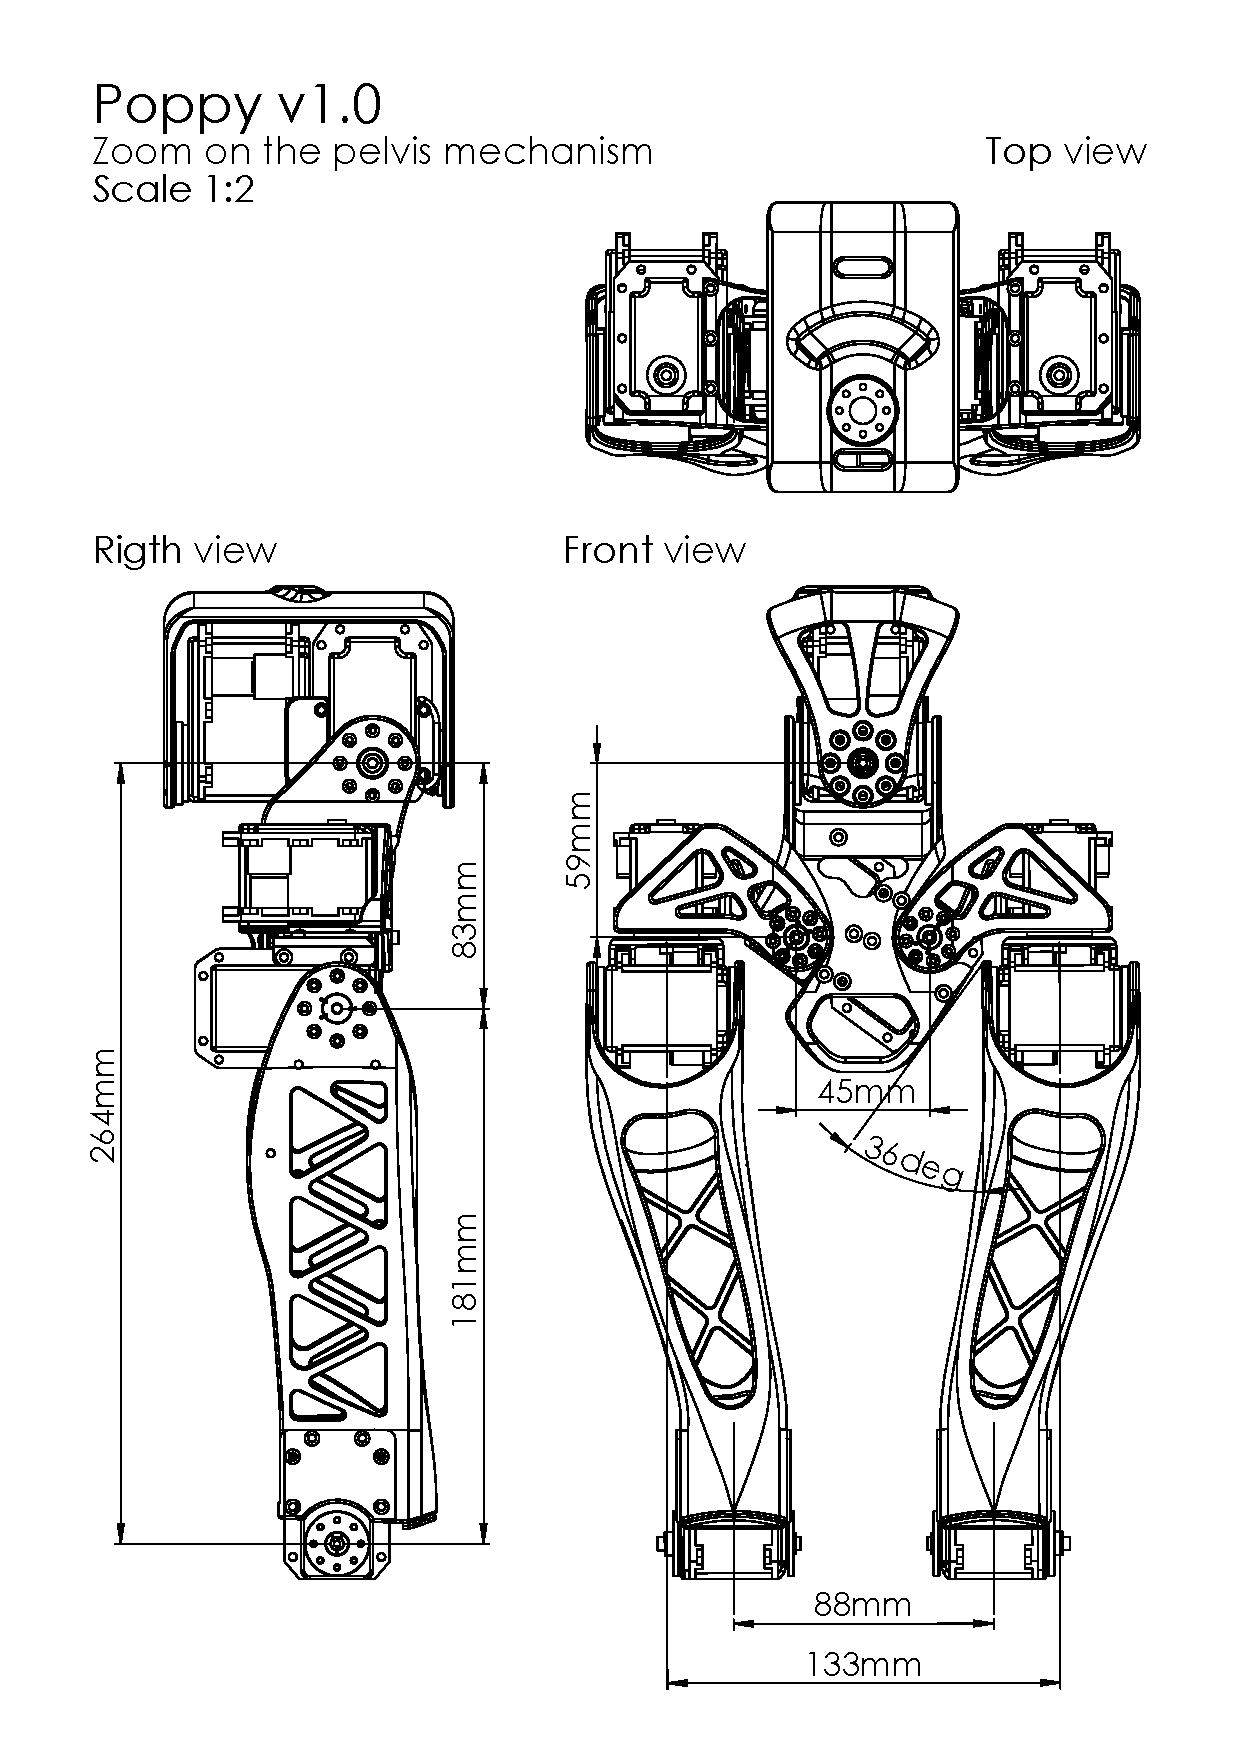
\includegraphics[width=\linewidth]{poppy_zoom_hip_blueprint.pdf}
    \end{center}
    \caption{This blueprint shows the design of Poppy's pelvis. The use of a non-symmetrical configuration of motors permits to embed 6 DoFs in a compact space while keeping a wide range of motion in all direction.}
    \label{fig:poppy_zoom_hip_blueprint}
\end{figure}

In addition, to reduce the shifting of the center of gravity to the back of the robot, the connection with the abs motors is slightly shifted toward the front. By doing so, we.
This enables us to keep the CoG within the support polygon and to increase the range of motion of the abs motor when the robot leans forward.


\section{Multi-articulated torso} % (fold)

Humanoid robots mostly have a rigid torso without any joints (e.g DarwinOp, Nao, NimbroOP) or few DoFs (e.g. two for iCub, one for HRP-2). However, if we look at the human trunk and in particular at the spine, it has a complex mechanical structure and a large network of dense muscles controlling a very large number of DoFs. It allows for complex motions in several directions while keeping balance. Its movements are regulated by a complex combination of anticipatory and reactive muscle actions.

Before 1982 and the work of Thorstensson~\parencite{thorstensson1982lumbar}, few scientists had really approached the subject. Since then, several studies have investigated the activity of the trunk during walking and showed that the trunk is not only an additional mass but, for example, participates actively in the human walk.
Electromyographic studies have shown the importance of the erector spinae muscles in the organization of motor patterns during walking~\parencite{anders2007trunk} but also of other rhythmic tasks~\parencite{de2008sequential}. Like the salamander~\parencite{ijspeert2007swimming}, a sequential activation of erector spinae muscles was found~\parencite{prince1994anticipatory}.
They also show that the trunk leans forward and oscillates from 1.5 to 6 degrees during walking. In addition, lateral flexion during a gait cycle on the frontal plane promotes the weight shift and opposite rotations of the lumbar and thoracic belts on the horizontal plane allow for the extension of the footstep (\cite{feipel2001three}, \cite{lamoth2006effects}).

\begin{figure}[ht]
    \begin{center}
        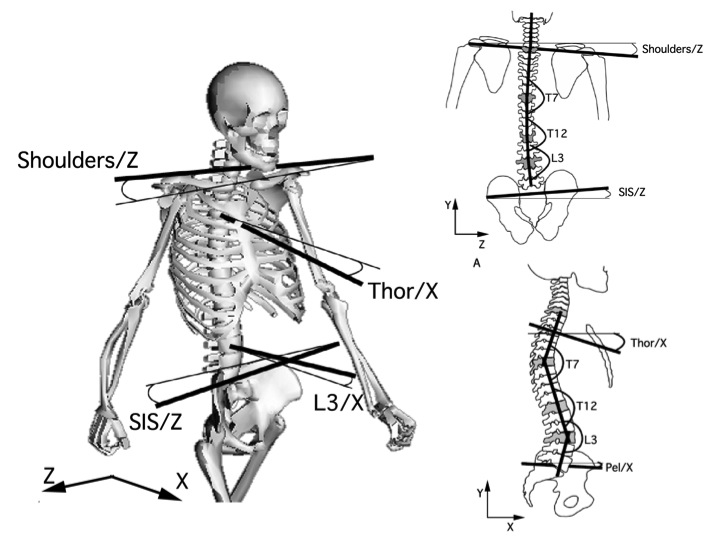
\includegraphics[width=0.7\linewidth]{human_trunk.jpg}
    \end{center}
    \caption{This figure shows the main human spine mobility in horizontal, frontal and sagittal plane. Figure extracted from~\parencite{ceccatoPlos09}}
    \label{fig:human_spine_system}
\end{figure}

Thus, the human torso is complex and seems to play an important role in walking; it is essential for all human movements but especially for walking. The movements of the spine can facilitate the transfer of weight from one leg to the other, improve the balance but also participate in the dynamics of walking.

It seems therefore interesting to equip a humanoid robot that is an attempt to explore the role of morphology, with an articulated trunk in order to evaluate its impact on several tasks, from dynamic walking to physical human-robot interaction. Yet the human torso is difficult to replicate on a small robot using servo motors and therefore simplification is needed.

Interestingly, Ceccato~\parencite{ceccatoPlos09} studied the role of the trunk during walking and highlighted that there are some places in the spine where the displacements are the most important, i.e. that the apparent high dimensionality of the trunk could be factorized down to a few essential components/dimensions.

Accordingly, it appears we can replicate the essential degrees of freedom of human torso with two DoFs on the sagittal plane, two on the coronal plane, placed in the pelvis and shoulder/thoracic and one on the horizontal plane placed in the middle of his torso.

These main degrees of freedom have been first introduced on Acroban~\parencite{ly2011bio} and continued on Poppy (see \figurename~\ref{fig:poppy_torso}).
Thus Poppy's trunk involves five degrees of freedom, we use two Dynamixel MX-64 for the abs as they have to support and move the whole upper body mass, the 3 others joints being less subject to high constraints are powered by MX-28 (see \figurename~\ref{fig:torso_blueprint}). This multi-articulated trunk allows a wide range of motion that can be useful to explore the role of the torso’s motion on complex dynamics behavior (balance, walking), grasping and reaching task, or for human-robot interaction, extending to the expressive and emotional abilities.

\begin{figure}[p]
\centering
    \subfloat{\label{fig:torso_blueprint}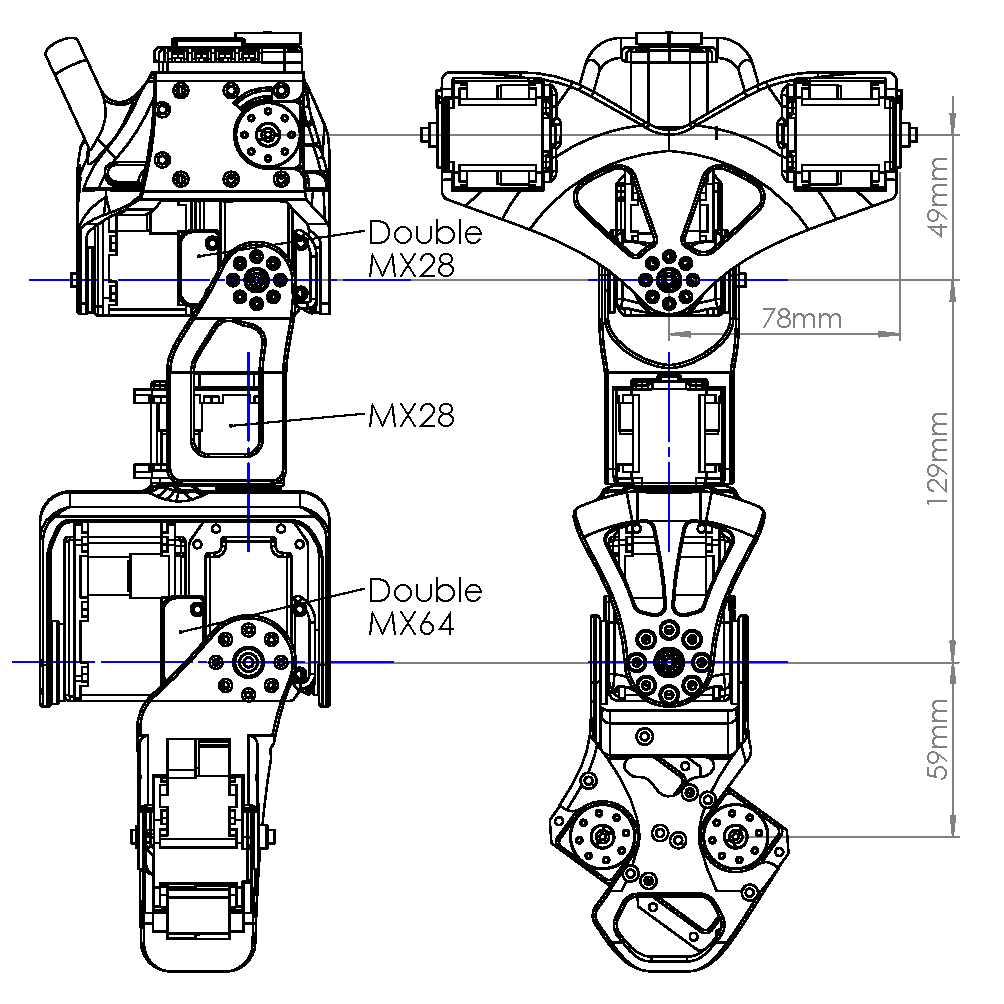
\includegraphics[width=0.95\linewidth]{poppy_torso.pdf}}


    \subfloat{\label{fig:frontal_trunk}\includegraphics[width=0.48\linewidth]{trunk_face.png}}
    \hfill
    \subfloat{\label{fig:sagittal_trunk}\includegraphics[width=0.48\linewidth]{trunk_sagittal.png}}
    \caption{This figure shows the blueprint of Poppy's 5 DoF torso as well as illustration of the resulting mobility.}
    \label{fig:poppy_torso}
\end{figure}



\subsection{Upper limbs} % (fold)

Poppy's arms were not designed for exploring grasping but rather for balancing, expressive and interactive purposes. Thus, they only involve the minimum articulations required to produce a wide range of movements and they do not involve articulated hands.

A first version of the robot arms involved low-cost AX-12 motors(\$50), but these motors do not allow the same degree of compliance as MX-28 so the interaction was not smooth enough. We quickly replaced them with MX-28 motors, even if they are more expensive (\$250), powerful and heavy (72gr rather than 50gr), the compliance ability is needed for playful physical interaction and demonstration.

This ability was especially useful for the experiments we made with Poppy walking while being socially guided by its hands\footnote{see video \url{https://vimeo.com/74557773}} and experiments on chapter~\ref{cha:changing_morphology}.

Also, these arms combined with the complex spine make Poppy a particularly adapted tool for creating and studying emotions and gestural social communication (see \figurename~\ref{fig:TER_cognitic}). An example of such use has been demonstrated by two Cognitics students. Their goal was to study the transfer of emotion between robots and humans. Using Poppy's upper body and the pypot recording feature (see section~\ref{sub:move_recording}), they were able to program a wide range of emotions (see \figurename~\ref{fig:TER_cognitic}).


\begin{figure}[tb]
\centering
    \subfloat[][\url{http://youtu.be/StFIMuyz11M}]{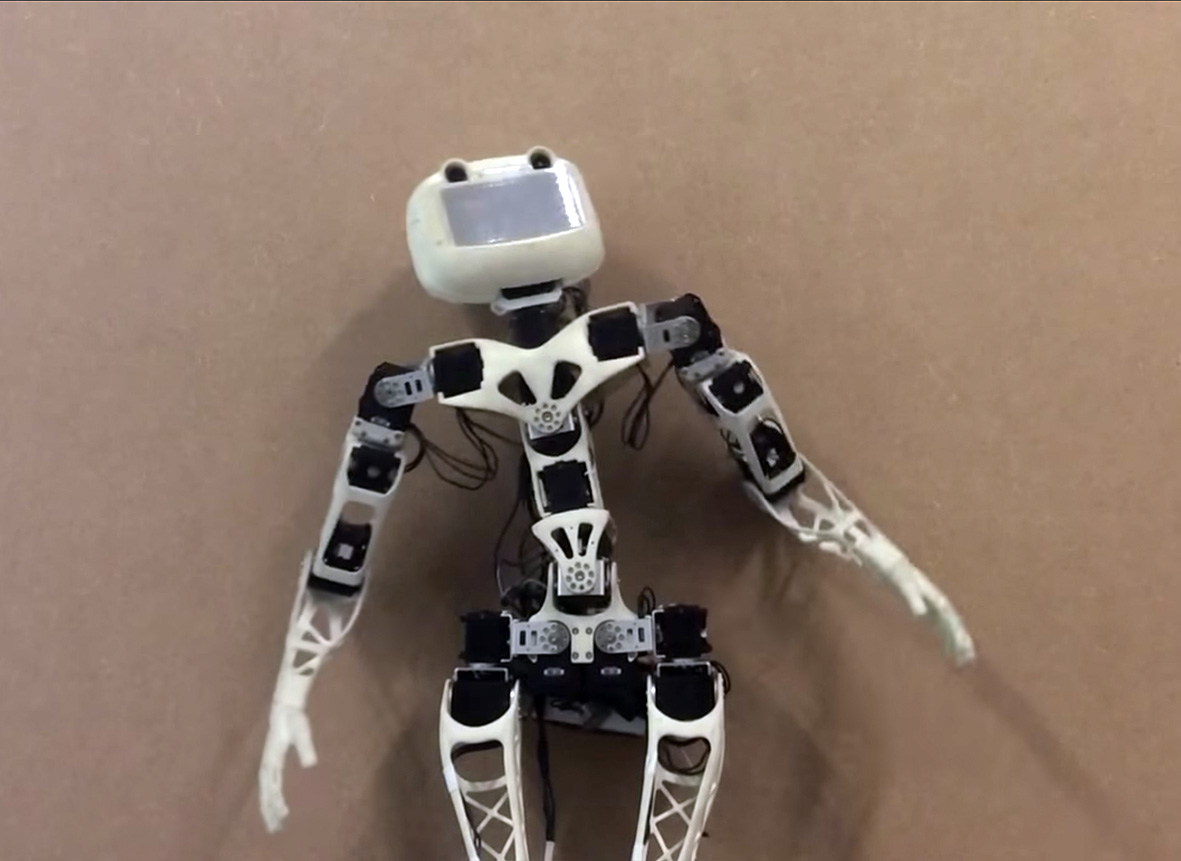
\includegraphics[width=0.45\linewidth]{TER_surprise.jpg}}
    \hfil
    \subfloat[][\url{http://youtu.be/RwCtNwLk10E}]{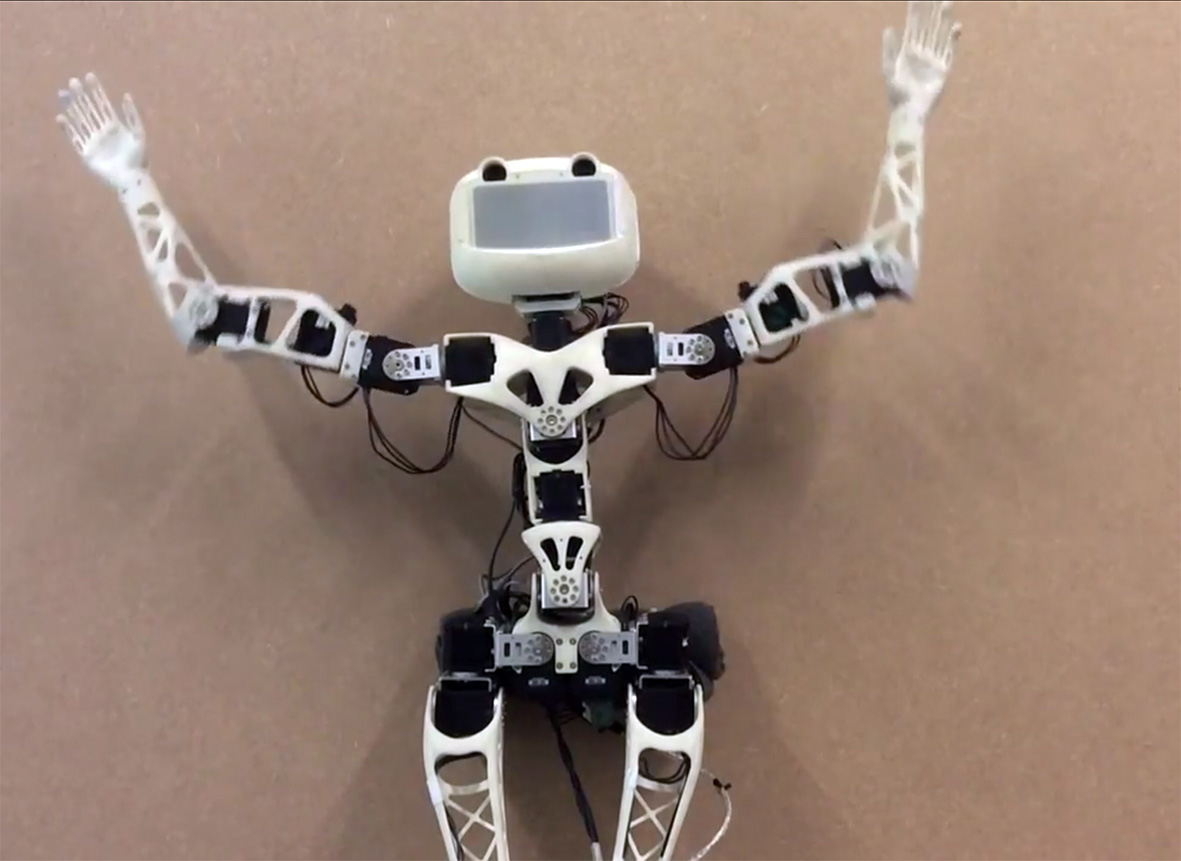
\includegraphics[width=0.45\linewidth]{TER_joy.jpg}}\\
    \subfloat[][\url{http://youtu.be/qrcmLXbpUVo}]{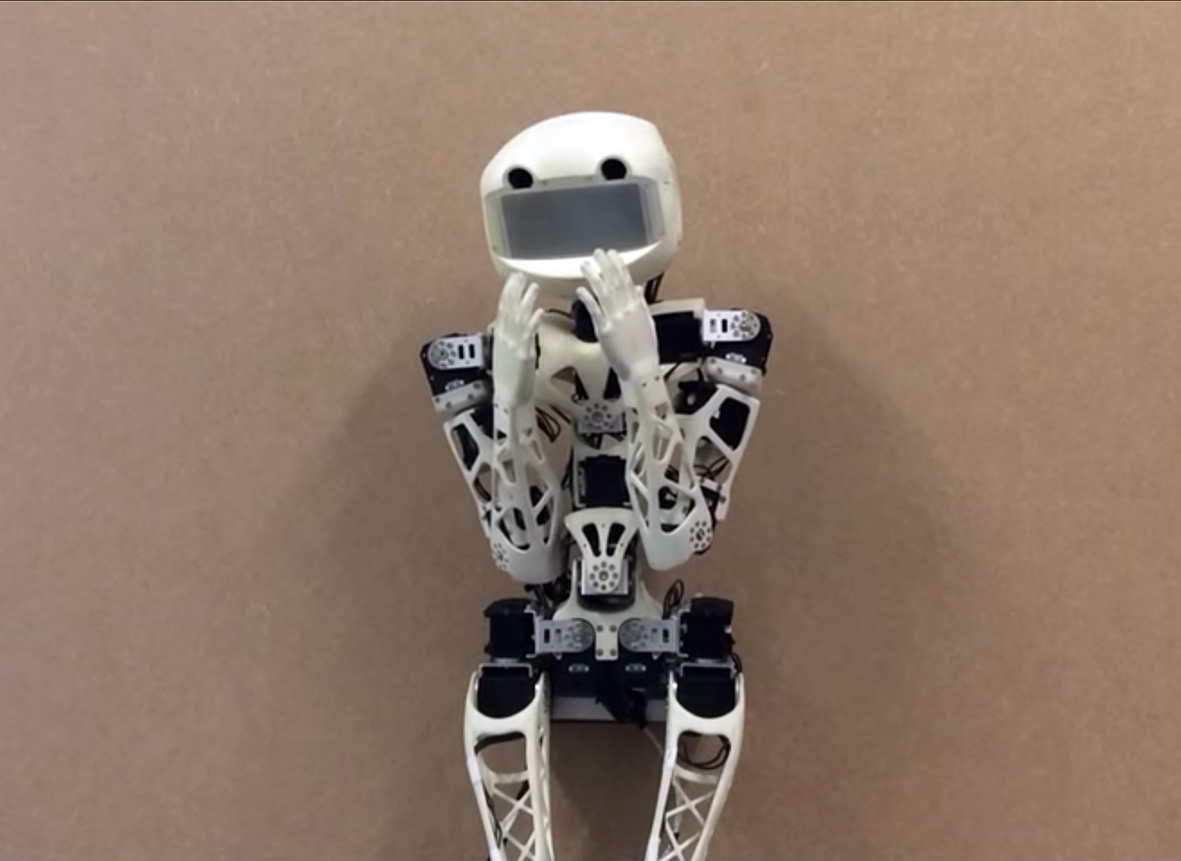
\includegraphics[width=0.45\linewidth]{TER_sad.jpg}}
    \hfil
    \subfloat[][\url{http://youtu.be/ms2niFLevv8}]{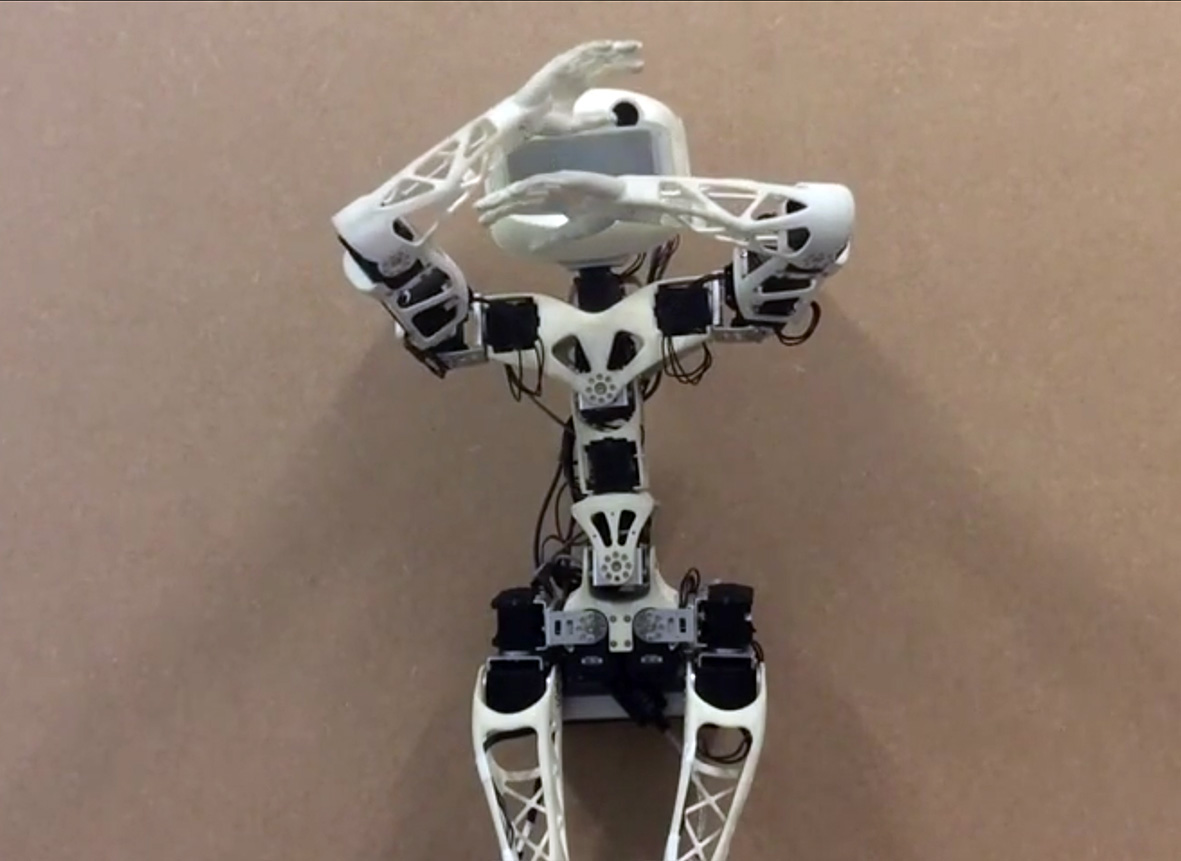
\includegraphics[width=0.45\linewidth]{TER_fear.jpg}}
    \caption{The upper body mobility of Poppy allows for rich exploration of humanoid robot behaviour. Cognitics students have used Poppy to create and explore robotic emotion and study how people react. Using the multi-articulated torso and arms, they created a wide range of emotion those video links is displayed under each illustration. }
    \label{fig:TER_cognitic}
\end{figure}


